
%	-------------------------------------------------------------------------------
% 
%
%
%		붓다의 일생
%
%		2022.07.20.수  첫 작
%
%
%
%
%	-------------------------------------------------------------------------------

	\documentclass[12pt, a4paper, oneside]{book}
%	\documentclass[12pt, a4paper, landscape, oneside]{book}

		% --------------------------------- 페이지 스타일 지정
		\usepackage{geometry}
%		\geometry{landscape=true	}
		\geometry{top 		=10em}
		\geometry{bottom		=10em}
		\geometry{left		=8em}
		\geometry{right		=8em}
		\geometry{headheight	=4em} % 머리말 설치 높이
		\geometry{headsep		=2em} % 머리말의 본문과의 띠우기 크기
		\geometry{footskip		=4em} % 꼬리말의 본문과의 띠우기 크기
% 		\geometry{showframe}
	
%		paperwidth 	= left + width + right (1)
%		paperheight 	= top + height + bottom (2)
%		width 		= textwidth (+ marginparsep + marginparwidth) (3)
%		height 		= textheight (+ headheight + headsep + footskip) (4)



		%	===================================================================
		%	package
		%	===================================================================
%			\usepackage[hangul]{kotex}				% 한글 사용
			\usepackage{kotex}					% 한글 사용
			\usepackage[unicode]{hyperref}			% 한글 하이퍼링크 사용

		% ------------------------------ 수학 수식
			\usepackage{amssymb,amsfonts,amsmath}	% 수학 수식 사용
			\usepackage{mathtools}				% amsmath 확장판

			\usepackage{scrextend}				% 
		

		% ------------------------------ LIST
			\usepackage{enumerate}			%
			\usepackage{enumitem}			%
			\usepackage{tablists}				%	수학문제의 보기 등을 표현하는데 사용
										%	tabenum


		% ------------------------------ table 
			\usepackage{longtable}			%
			\usepackage{tabularx}			%
			\usepackage{tabu}				%




		% ------------------------------ 
			\usepackage{setspace}			%
			\usepackage{booktabs}		% table
			\usepackage{color}			%
			\usepackage{multirow}			%
			\usepackage{boxedminipage}	% 미니 페이지
			\usepackage[pdftex]{graphicx}	% 그림 사용
			\usepackage[final]{pdfpages}		% pdf 사용
			\usepackage{framed}			% pdf 사용

			
			\usepackage{fix-cm}	
			\usepackage[english]{babel}

		% ------------------------------ 음악
%			\usepackage{kslilymusic}			%
%			\usepackage{lyluatex}
	
		%	=======================================================================================
		% 	tikz package
		% 	
		% 	--------------------------------- 	
			\usepackage{tikz}%
			\usetikzlibrary{arrows,positioning,shapes}
			\usetikzlibrary{mindmap}			
			

		% --------------------------------- 	page
			\usepackage{afterpage}		% 다음페이지가 나온면 어떻게 하라는 명령 정의 패키지
%			\usepackage{fullpage}			% 잘못 사용하면 다 흐트러짐 주의해서 사용
%			\usepackage{pdflscape}		% 
			\usepackage{lscape}			%	 


			\usepackage{blindtext}
	
		% --------------------------------- font 사용
			\usepackage{pifont}				%
			\usepackage{textcomp}
			\usepackage{gensymb}
			\usepackage{marvosym}



		% Package --------------------------------- 

			\usepackage{tablists}				%


		% Package --------------------------------- 
			\usepackage[framemethod=TikZ]{mdframed}				% md framed package
			\usepackage{smartdiagram}								% smart diagram package



		% Package ---------------------------------    연습문제 

			\usepackage{exsheets}				%

			\SetupExSheets{solution/print=true}
			\SetupExSheets{question/type=exam}
			\SetupExSheets[points]{name=point,name-plural=points}


		% --------------------------------- 페이지 스타일 지정

		\usepackage[Sonny]		{fncychap}

			\makeatletter
			\ChNameVar	{\Large\bf}
			\ChNumVar	{\Huge\bf}
			\ChTitleVar		{\Large\bf}
			\ChRuleWidth	{0.5pt}
			\makeatother

%		\usepackage[Lenny]		{fncychap}
%		\usepackage[Glenn]		{fncychap}
%		\usepackage[Conny]		{fncychap}
%		\usepackage[Rejne]		{fncychap}
%		\usepackage[Bjarne]	{fncychap}
%		\usepackage[Bjornstrup]{fncychap}

		\usepackage{fancyhdr}
		\pagestyle{fancy}
		\fancyhead{} % clear all fields
		\fancyhead[LO]{\footnotesize \leftmark}
		\fancyhead[RE]{\footnotesize \leftmark}
		\fancyfoot{} % clear all fields
		\fancyfoot[LE,RO]{\large \thepage}
		%\fancyfoot[CO,CE]{\empty}
		\renewcommand{\headrulewidth}{1.0pt}
		\renewcommand{\footrulewidth}{0.4pt}
	
	
	
		%	--------------------------------------------------------------------------------------- 
		% 	tritlesec package
		% 	
		% 	
		% 	------------------------------------------------------------------ section 스타일 지정
	
			\usepackage{titlesec}
		
		% 	----------------------------------------------------------------- section 글자 모양 설정
			\titleformat*{\section}					{\large\bfseries}
			\titleformat*{\subsection}				{\normalsize\bfseries}
			\titleformat*{\subsubsection}			{\normalsize\bfseries}
			\titleformat*{\paragraph}				{\normalsize\bfseries}
			\titleformat*{\subparagraph}				{\normalsize\bfseries}
	
		% 	----------------------------------------------------------------- section 번호 설정
			\renewcommand{\thepart}				{\arabic{part}.}
			\renewcommand{\thesection}				{\arabic{section}.}
			\renewcommand{\thesubsection}			{\thesection\arabic{subsection}.}
			\renewcommand{\thesubsubsection}		{\thesubsection\arabic{subsubsection}}
			\renewcommand\theparagraph 			{$\blacksquare$ \hspace{3pt}}

		% 	----------------------------------------------------------------- section 페이지 나누기 설정
			\let\stdsection\section
			\renewcommand\section{\newpage\stdsection}



		%	--------------------------------------------------------------------------------------- 
		% 	\titlespacing*{commandi} {left} {before-sep} {after-sep} [right-sep]		
		% 	left
		%	before-sep		:  수직 전 간격
		% 	after-sep	 	:  수직으로 후 간격
		%	right-sep

			\titlespacing*{\section} 			{0pt}{1.0em}{1.0em}
			\titlespacing*{\subsection}	  		{0ex}{1.0em}{1.0em}
			\titlespacing*{\subsubsection}		{0ex}{1.0em}{1.0em}
			\titlespacing*{\paragraph}			{0em}{1.5em}{1.0em}
			\titlespacing*{\subparagraph}		{4em}{1.0em}{1.0em}
	
		%	\titlespacing*{\section} 			{0pt}{0.0\baselineskip}{0.0\baselineskip}
		%	\titlespacing*{\subsection}	  		{0ex}{0.0\baselineskip}{0.0\baselineskip}
		%	\titlespacing*{\subsubsection}		{6ex}{0.0\baselineskip}{0.0\baselineskip}
		%	\titlespacing*{\paragraph}			{6pt}{0.0\baselineskip}{0.0\baselineskip}
	

		% --------------------------------- recommend		섹션별 페이지 상단 여백
		\newcommand{\SectionMargin}				{\newpage  \null \vskip 2cm}
		\newcommand{\SubSectionMargin}			{\newpage  \null \vskip 2cm}
		\newcommand{\SubSubSectionMargin}		{\newpage  \null \vskip 2cm}


		%	--------------------------------------------------------------------------------------- 
		% 	toc 설정  - table of contents
		% 	
		% 	
		% 	----------------------------------------------------------------  문서 기본 사항 설정
			\setcounter{secnumdepth}{4} 		% 문단 번호 깊이
			\setcounter{tocdepth}{2} 			% 문단 번호 깊이 - 목차 출력시 출력 범위

			\setlength{\parindent}{0cm} 		% 문서 들여 쓰기를 하지 않는다.


		%	--------------------------------------------------------------------------------------- 
		% 	mini toc 설정
		% 	
		% 	
		% 	--------------------------------------------------------- 장의 목차  minitoc package
			\usepackage{minitoc}

			\setcounter{minitocdepth}{1}    	%  Show until subsubsections in minitoc
%			\setlength{\mtcindent}{12pt} 	% default 24pt
			\setlength{\mtcindent}{24pt} 	% default 24pt

		% 	--------------------------------------------------------- part toc
		%	\setcounter{parttocdepth}{2} 	%  default
			\setcounter{parttocdepth}{0}
		%	\setlength{\ptcindent}{0em}		%  default  목차 내용 들여 쓰기
			\setlength{\ptcindent}{0em}         


		% 	--------------------------------------------------------- section toc

			\renewcommand{\ptcfont}{\normalsize\rm} 		%  default
			\renewcommand{\ptcCfont}{\normalsize\bf} 	%  default
			\renewcommand{\ptcSfont}{\normalsize\rm} 	%  default


		%	=======================================================================================
		% 	tocloft package
		% 	
		% 	------------------------------------------ 목차의 목차 번호와 목차 사이의 간격 조정
			\usepackage{tocloft}

		% 	------------------------------------------ 목차의 내어쓰기 즉 왼쪽 마진 설정
			\setlength{\cftsecindent}{2em}			%  section

		% 	------------------------------------------ 목차의 목차 번호와 목차 사이의 간격 조정
			\setlength{\cftsecnumwidth}{2em}		%  section





		%	=======================================================================================
		% 	flowchart  package
		% 	
		% 	------------------------------------------ 목차의 목차 번호와 목차 사이의 간격 조정
			\usepackage{flowchart}
			\usetikzlibrary{arrows}



		%	=======================================================================================
		% 	줄 간격 설정
		% 	
		% 	
		% 	--------------------------------- 	줄간격 설정
			\doublespace
%			\onehalfspace
%			\singlespace
		
		

	% 	============================================================================== itemi Global setting

	
		%	-------------------------------------------------------------------------------
		%		Vertical spacing
		%	-------------------------------------------------------------------------------
			\setlist[itemize]{topsep=0.0em}			% 상단의 여유치
			\setlist[itemize]{partopsep=0.0em}			% 
			\setlist[itemize]{parsep=0.0em}			% 
%			\setlist[itemize]{itemsep=0.0em}			% 
			\setlist[itemize]{noitemsep}				% 
			
		%	-------------------------------------------------------------------------------
		%		Horizontal spacing
		%	-------------------------------------------------------------------------------
			\setlist[itemize]{labelwidth=1em}			%  라벨의 표시 폭
			\setlist[itemize]{leftmargin=8em}			%  본문 까지의 왼쪽 여백  - 4em
			\setlist[itemize]{labelsep=3em} 			%  본문에서 라벨까지의 거리 -  3em
			\setlist[itemize]{rightmargin=0em}			% 오른쪽 여백  - 4em
			\setlist[itemize]{itemindent=0em} 			% 점 내민 거리 label sep 과 같은면 점위치 까지 내민다
			\setlist[itemize]{listparindent=3em}		% 본문 드려쓰기 간격
	
	
			\setlist[itemize]{ topsep=0.0em, 			%  상단의 여유치
						partopsep=0.0em, 		%  
						parsep=0.0em, 
						itemsep=0.0em, 
						labelwidth=1em, 
						leftmargin=2.5em,
						labelsep=2em,			%  본문에서 라벨 까지의 거리
						rightmargin=0em,		% 오른쪽 여백  - 4em
						itemindent=0em, 		% 점 내민 거리 label sep 과 같은면 점위치 까지 내민다
						listparindent=0em}		% 본문 드려쓰기 간격
	
%			\begin{itemize}
	
		%	-------------------------------------------------------------------------------
		%		Label
		%	-------------------------------------------------------------------------------
			\renewcommand{\labelitemi}{$\bullet$}
			\renewcommand{\labelitemii}{$\bullet$}
%			\renewcommand{\labelitemii}{$\cdot$}
			\renewcommand{\labelitemiii}{$\diamond$}
			\renewcommand{\labelitemiv}{$\ast$}		
	
%			\renewcommand{\labelitemi}{$\blacksquare$}   	% 사각형 - 찬것
%			\renewcommand\labelitemii{$\square$}		% 사각형 - 빈것	
			






% ------------------------------------------------------------------------------
% Begin document (Content goes below)
% ------------------------------------------------------------------------------
	\begin{document}
	
			\dominitoc
			\doparttoc			



			\title{붓다의 일생}
			\author{김대희}
			\date{2022년 7월}
			\maketitle


			\tableofcontents 		% 목차 출력
%			\listoffigures 			% 그림 목차 출력
			\cleardoublepage
			\listoftables 			% 표 목차 출력





		\mdfdefinestyle	{con_specification} {
						outerlinewidth		=1pt			,%
						innerlinewidth		=2pt			,%
						outerlinecolor		=blue!70!black	,%
						innerlinecolor		=white 			,%
						roundcorner			=4pt			,%
						skipabove			=1em 			,%
						skipbelow			=1em 			,%
						leftmargin			=0em			,%
						rightmargin			=0em			,%
						innertopmargin		=2em 			,%
						innerbottommargin 	=2em 			,%
						innerleftmargin		=1em 			,%
						innerrightmargin		=1em 			,%
						backgroundcolor		=gray!4			,%
						frametitlerule		=true 			,%
						frametitlerulecolor	=white			,%
						frametitlebackgroundcolor=black		,%
						frametitleaboveskip=1em 			,%
						frametitlebelowskip=1em 			,%
						frametitlefontcolor=white 			,%
						}



%	================================================================== Part			요가 개요
%	\addtocontents{toc}{\protect\newpage}
	\part{붓다의 일생}
	\noptcrule
	\parttoc				

% -----------------------------------------------------------------------------
%
%
%
% -----------------------------------------------------------------------------
\chapter{탄생과 성장}


% -----------------------------------------------------------------------------
%
% -----------------------------------------------------------------------------
	\section{이 땅에 오시기까지 14 }


			\begin{center}
			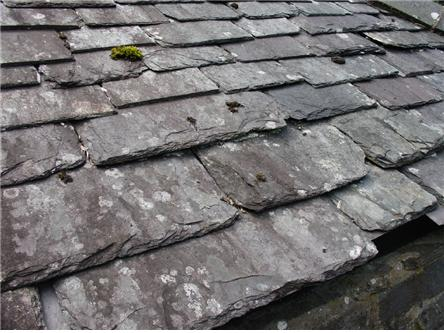
\includegraphics[width=0.8\textwidth]{./fig/slate_0001.jpg}
			\end{center}


% -----------------------------------------------------------------------------
%
% -----------------------------------------------------------------------------
	\section{하늘나라 도솔천 21 }

% -----------------------------------------------------------------------------
%
% -----------------------------------------------------------------------------
	\section{거룩한 탄생 25 }

% -----------------------------------------------------------------------------
%
% -----------------------------------------------------------------------------
	\section{선인의 예언 33 }

% -----------------------------------------------------------------------------
%
% -----------------------------------------------------------------------------
	\section{태자 싯닷타 36 }

% -----------------------------------------------------------------------------
%
% -----------------------------------------------------------------------------
	\section{잠부나무 아래에서의 선정 39 }

% -----------------------------------------------------------------------------
%
% -----------------------------------------------------------------------------
	\section{ 태자비 야소다라 42 }

% -----------------------------------------------------------------------------
%
% -----------------------------------------------------------------------------
	\section{호화로운 궁중 생활과 성문 밖의 고통 48 }

% -----------------------------------------------------------------------------
%
% -----------------------------------------------------------------------------
	\section{새로운 희망과 라훌라의 탄생 54}




%	================================================================== Part	제2장 구도의 길
%	\addtocontents{toc}{\protect\newpage}
	\chapter{구도의 길}
	\noptcrule
	\parttoc			


	\section{집을 나서다 60 }

	\section{슬픔에 젖은 까삘라왓투 65 }

	\section{숫도다나왕의 설득 68 }

	\section{스승을 찾아 웨살리로 71 }

	\section{빔비사라왕의 제안 77 }

	\section{사문들의 도시 라자가하 79 }

	\section{고행의 길 85 }

	\section{고행을 버리다 92	}





%	================================================================== Part 제3장 가장 높고 바른 깨달음
%	\addtocontents{toc}{\protect\newpage}
	\chapter{가장 높고 바른 깨달음}
	\noptcrule
	\parttoc				

	\section{수자따의 우유죽 96 }

	\section{보리수 아래에서 98 }

	\section{마라의 유혹과 위협 100 }

	\section{깨달음 107 }

	\section{천인들의 축복 110 }

	\section{성도 후 49일 113 }

	\section{범천의 권청 117}





%	================================================================== Part	제4장 전법의 길
%	\addtocontents{toc}{\protect\newpage}
	\chapter{제4장 전법의 길}
	\noptcrule
	\parttoc				

	\section{와라나시로 가는 길 124 }

	\section{녹야원의 다섯 수행자 127 }

	\section{야사의 귀의 135 }

	\section{법을 전하라 140 }

	\section{깟사빠 삼형제의 제도 144 }

	\section{가야산 꼭대기에서 150}





%	================================================================== Part		제5장 교화의 터전 라자가하
%	\addtocontents{toc}{\protect\newpage}
	\chapter{제5장 교화의 터전 라자가하}
	\noptcrule
	\parttoc				

	\section{죽림정사 154 }

	\section{사리뿟따와 마하목갈라나의 귀의 160 }

	\section{시기와 질투 165 }

	\section{마하깟사빠의 귀의 169 }

	\section{계율의 제정 173}





%	================================================================== Part	제6장 고향에서의 전법
%	\addtocontents{toc}{\protect\newpage}
	\chapter{제6장 고향에서의 전법}
	\noptcrule
	\parttoc				

	\section{부왕의 초대 180 }

	\section{다시 찾은 까삘라왓투 186 }

	\section{고향에서의 걸식 191 }

	\section{야소다라와의 재회 194 }

	\section{난다의 출가 197 }

	\section{라훌라의 출가 201 }

	\section{왕자들의 출가 204}





%	================================================================== Part	제7장 교단의 성장
%	\addtocontents{toc}{\protect\newpage}
	\chapter{제7장 교단의 성장}
	\noptcrule
	\parttoc				

	\section{사왓티의 상인 수닷따 210 }

	\section{기원정사의 건립 215 }

	\section{빠세나디왕의 귀의 220 }

	\section{웨살리 재앙의 퇴치 229 }

	\section{사꺄족과 꼴리야족의 물싸움 234 }

	\section{숫도다나왕의 임종과 비구니 승가의 탄생 242 }

	\section{왕비 케마의 출가 250 }

	\section{꼬삼비의 세 정사 257 }

	\section{남쪽 아완띠까지 262}



%	================================================================== Part	제8장 지혜와 자비의 가르침
%	\addtocontents{toc}{\protect\newpage}
	\chapter{제8장 지혜와 자비의 가르침}
	\noptcrule
	\parttoc				


	\section{붉은 옷을 입은 찐짜 266 }

	\section{악기를 연주하듯 273 }

	\section{과거생의 부모님 274 }

	\section{꼬삼비 분쟁 281 }

	\section{마음 밭의 경작 287 }

	\section{웨란자에서의 안거 292 }

	\section{소치는 다니야 296 }

	\section{행복과 파멸의 문 301 }

	\section{죽은 아들과 겨자씨 304}




%	================================================================== Part	제9장 평화와 평등의 가르침
%	\addtocontents{toc}{\protect\newpage}
	\chapter{제9장 평화와 평등의 가르침}
	\noptcrule
	\parttoc				


	\section{시자 아난다 312 }

	\section{진리의 어머니 위사카 316 }

	\section{사리뿟따의 사자후 321 }

	\section{살인자 앙굴리말라 326 }

	\section{통을 지던 니디 338 }

	\section{누더기를 걸친 마하깟사빠 342 }

	\section{시체를 태우는 막대기들 346 }

	\section{데와닷따의 반역 349 }

	\section{아자따삿뚜의 참회 358}


%	================================================================== Part	제10장 마지막 유행
%	\addtocontents{toc}{\protect\newpage}
	\chapter{제10장 마지막 유행}
	\noptcrule
	\parttoc				


	\section{파멸하지 않는 일곱 가지 법 370 }

	\section{강가강을 건너 웨살리로 373 }

	\section{벨루와에서의 안거 377 }

	\section{마지막 공양과 마지막 가사 382 }

	\section{두 그루 살라나무 아래에서 388 }

	\section{마지막 제자 수밧다 392 }

	\section{등불은 꺼지고 396 }

	\section{다비와 불사리탑 400 }

	\section{인류의 영원한 스승 408}


%	================================================================== Part	부록
%	\addtocontents{toc}{\protect\newpage}
	\chapter{부록}
	\noptcrule
	\parttoc				


	\section{부처님 가계도 422}


	\section{부처님 일생 연표 424 }

	\section{부처님 재세 시 16국과 설법 장소 426}


	\section{부처님 재세 시 강가강 유역 428 }

	\section{부처님 안거 장소 430 }

	\section{불기 산정 기준 432 }

	\section{인도불교사 연표 433 }

	\section{인명·지명 대조표 436 }

	\section{불전도 해설 448 }

	\section{참고자료 459}

	\section{색인 463 }

	\section{방함록 470}


% ------------------------------------------------------------------------------
% End document
% ------------------------------------------------------------------------------
\end{document}



% =================================================================================================== Part 혼화 재료

% ========================================================================================= chapter

%	-----------------------------------------------------------  section  

	%	------------------------------------------------------------------------------  table

			\begin{table} [h]
	
			\caption{잔 골재의 표준입도}  
			\label{tab:title} 
	
			\begin{center}
			\tabulinesep=0.4em
			\begin{tabu} to 0.8\linewidth { X[r] X[l] X[c]  }
			\tabucline [1pt,] {-}
			체의 호칭 치수 (mm)		& 체를 통화한 것의 질량 백분율(\%) \\
			\multicolumn{4}{c} {단위량} \\
			\tabucline [0.1pt,] {-}
			2.5	&100\\
			1.2	& 99 $\sim$ 100 \\
			0.6	& 60 $\sim$ 80 \\
			0.3	& 20 $\sim$ 50 \\
			0.15	&  5 $\sim$ 30 \\
			\tabucline [0.1pt,] {-}
			\end{tabu} 
			\end{center}
			\end{table}



	%	------------------------------------------------------------------------------  문제

		\clearpage
		\begin{small}	
		\begin{question}
		레디 믹스트 콘크리트에서 \textbf{회수수}를 혼합수로 사용할 경우 주의할 사항 중 틀린것은 ?
		\begin{enumerate}[label=\arabic*), topsep=0.0em, itemsep=-1.0em ]
			\item [①] 고강도 콘크리트의 경우 회수수를 사용하여서는 안된다. 
			\item [②] 슬러지수의 사용 시 \textbf{단위 슬러지 고형분}은 콘크리트 질량의 3\% 이하로 한다. 
			\item [③] 회수수의 품질 시험 항목은 4가지로 염소 이온량, 시멘트 응결 시간의 차, 모르타르 압축강도의 비, 단위 슬러지 고형분율 이다. 
			\item [④] 콘크리트를 배합할 때, 회수수 중에 함유된 슬러지 고형분은 물의 질량에는 포함되지 않는다. 
		\end{enumerate}
		\end{question}



		\begin{solution}
		해설
		\end{solution}
		\end{small}	
		\hrulefill


		%	----------------------------------------------------------------------------- 수식
			\begin{equation}
			\begin{aligned}
			T_2 = T_1 - 0.15 ( T_1 - T_0 ) \times t
			\end{aligned}
			\end{equation}


			\begin{description}[style=sameline, leftmargin=2cm, topsep=0.0em, itemsep=0.0em]
			\item[$T_0$] 		주의의 온도(${}^\circ C$)
			\item[$T_1$] 		비볐을때의 콘크리트 온도 (${}^\circ C$)
			\item[$t$] 		비빈후 부터 타설이 끝났을때 까지의 시간 (h)
			\end{description}



			\begin{itemize}[topsep=0.0em, parsep=0.0em, itemsep=0em, leftmargin=12.0em, labelwidth=3em, labelsep=3em] 
			\item [1.] 	따다 아사나
			\item [2.] 	우드르바 하스타 아사나
			\item [3.] 	웃따나 아사나
			\item [4.] 	아르다 웃따나 아사나
			\item [5.] 	차뚜랑가 단다 아사나
			\item [6.] 	우르드바 우카 스바나 아사나
			\item [7.] 	아도무카 스바나 아사나
			\item [8.] 	아르다 웃따나 아사나
			\item [9.] 	웃따나 아사나
			\item [10.] 	우드르바 하스타 아사나
			\item [11.] 	따다 아사나
			\end{itemize}


	\href{https://www.youtube.com/watch?v=SpqKCQZQBcc}{태양경배자세A}
	\href{https://www.youtube.com/watch?v=CL3czAIUDFY}{태양경배자세A}